\subsection{mediciones}
\frame{
	\frametitle{Mediciones de hist\'eresis}
	\begin{itemize}
		\item Medidas con un diodo l\'aser con $\lambda= ~660~nm.$
	\end{itemize}
	\begin{figure}[!hbt]
		\centering
		\subfigure[Rotaci\'on Kerr]{
			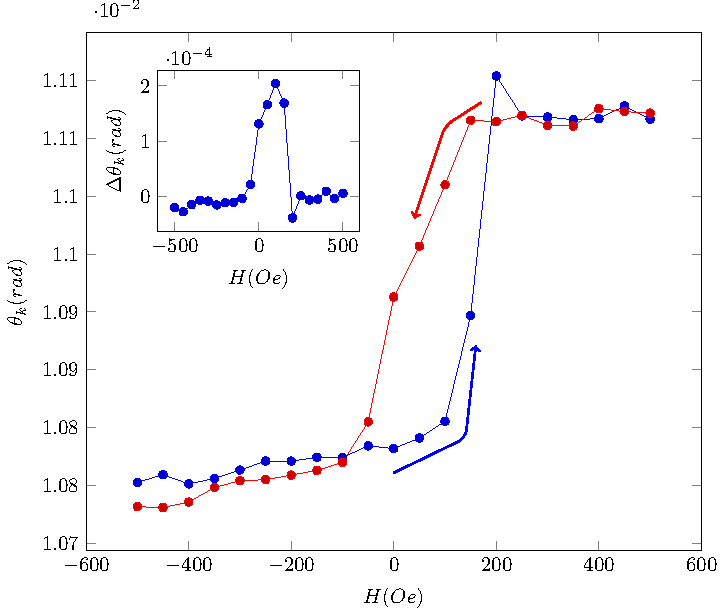
\includegraphics[scale=0.4]{resexp/his/HisTheta.pdf}
			\label{Exp:fig:theta}
		}
		\subfigure[Elipticidad Kerr]{
			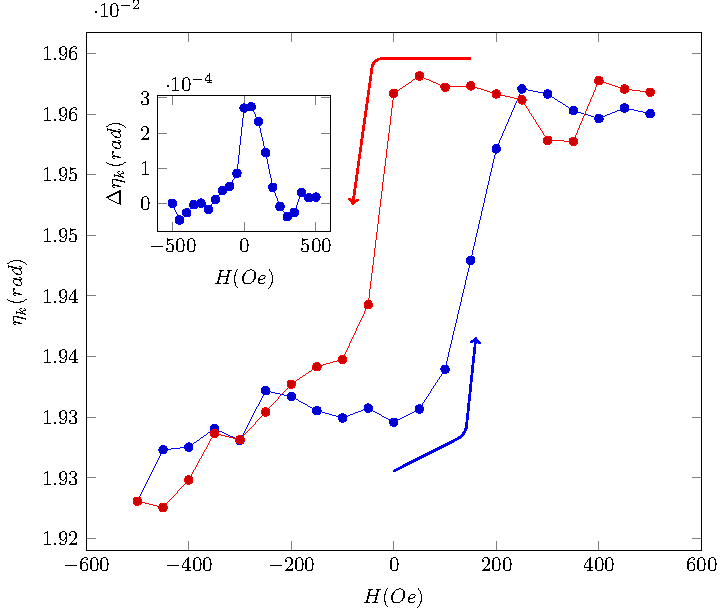
\includegraphics[scale=0.4]{resexp/his/HisEpsilon.pdf}
			\label{Exp:fig:elip}
		}
		\caption[Hit\'eresis de $\theta_k$ y $\eta_k$ en CoFeB]{Medici\'on de rotaci\'on (\ref{Exp:fig:theta}) y elipticidad (\ref{Exp:fig:elip}) Kerr enuna muestra de CoFeB. Dentro de cada figura se muestra en cambio de la se\~nal medida con cada direcci\'on de campo magn\'etico.}
		\label{Exp:fig:Kerrhis}
		
	\end{figure}
}
\frame{
\frametitle{Mediciones de espectro}
\begin{figure}[!hbt]
	\centering
	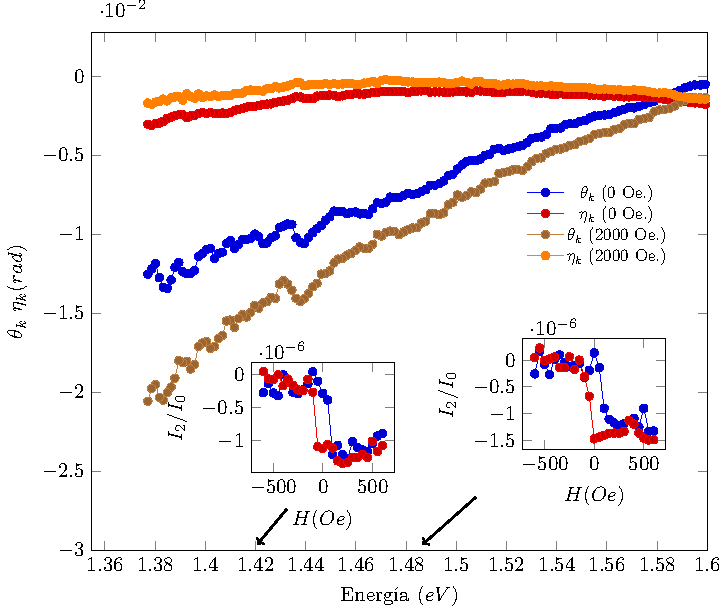
\includegraphics[scale=0.6]{resexp/esp/espectro0.pdf}
	\caption[Espectro de efecto Kerr magneto-\'optico]{Espectros del \'angulo y elipticidad Kerr en funci\'on de la energ\'ia del fot\'on en donde se induce un campo de $2000 Oe$. }
	\label{Exp:fig:espectroK}
\end{figure}
}